\chapter{Interface, Mass Ledger, CAD Export and Figures}\label{ch:s10-s12}

\lead{Stages S10, S11 and S12: from a solved engine state to joint checks, mass, exchange files and figures}

Stages \stagetag{S10}--\stagetag{S12} consume the results of S03--S09. \stagetag{S10} resolves and screens the bolted injector/chamber joint and, on one orchestrator only, prices hardware in a mass ledger; \stagetag{S11} writes stereolithography (STL) meshes, STEP (ISO~10303) boundary-representation (B-rep) solids and sidecar reports; \stagetag{S12} renders figures and animations. None feeds back into the contour, performance, cooling, injector or pump solutions; S10's write-back of the resolved flange and bolt dimensions into the arguments and the \code{InjectorSpec} happens after the injector solve, so only the throttle map, the CAD exporters and the interface screen read it. Two orchestrators run different S10 code: the command-line interface (CLI) path \code{raosim.run_nozzle.main} runs the interface resolver, the screen and all S11/S12 exporters, while \code{design.design_nozzle_v2} (legacy \code{main.py} batch-v2, MDO \code{--mdo-export}, the \texttt{lrekit run} re-evaluation) runs the interface screen without the composite-wall screen and is the only caller of the mass ledger. Every artifact that carries a release flag writes \texttt{hardware\_qualified = False}. Figure~\ref{fig:s10-s12-order} gives the hand-off order; line numbers refer to \code{raosim/run_nozzle.py} in the working tree of 2026-11-05.

\begin{figure}[tbp]
\centering
\begin{tikzpicture}[
  node distance=0.9mm,
  box/.style={draw=rulegray, fill=pale, rounded corners=1.2pt, align=left,
              font=\scriptsize\sffamily, text width=15.2cm, inner sep=1.6pt},
  tag/.style={font=\scriptsize\sffamily\bfseries, text=teal, anchor=east}]
\node[box] (p1) {:6212\quad \texttt{pumps.size\_electric\_pumps} (only \texttt{-{}-electric-pump}, which requires \texttt{-{}-injector pintle})};
\node[box, below=of p1] (p2) {:6239--6326\quad \texttt{pump\_cad.export\_pump\_package} $\rightarrow$ \texttt{pump/}; format \texttt{step|both} adds \texttt{pump\_cad\_brep} $\rightarrow$ \texttt{pump/pump\_brep/}};
\node[box, below=of p2] (p3) {:6327--6351\quad \texttt{flow\_viz.animate\_pump\_particles} $\rightarrow$ \texttt{pump\_particles.gif} (only \texttt{-{}-pump-visualize})};
\node[box, below=of p3] (i1) {:6369--6432\quad \texttt{resolve\_machined\_pintle\_layout} + \texttt{resolve\_bolted\_interface\_geometry}; write-back};
\node[box, below=of i1] (i2) {:6434--6510\quad \texttt{injector.throttle\_map} (only \texttt{-{}-throttle-map})};
\node[box, below=of i2] (i3) {:6512--6558\quad \texttt{injector\_export.export\_pintle\_package} $\rightarrow$ \texttt{pintle/}};
\node[box, below=of i3] (i4) {:6560--6571\quad \texttt{injector\_plots.export\_all\_injector\_figures} $\rightarrow$ \texttt{injector\_*.png}};
\node[box, below=of i4] (s1) {:6573--6655\quad \texttt{screen\_composite\_regen\_wall} (sized profile) + \texttt{screen\_injector\_chamber\_interface}; every run};
\node[box, below=of s1] (c1) {:6657--6878\quad \texttt{export\_stl}/\texttt{inspect\_stl}, \texttt{export\_step}, \texttt{export\_channel\_wall\_step}, \texttt{package\_ipt\_request}};
\node[box, below=of c1] (c2) {:6880--6904\quad \texttt{regen\_geometry.generate\_regen\_nozzle} $\rightarrow$ \texttt{regen.stl}, \texttt{regen\_3d.png} (only \texttt{-{}-regen})};
\node[box, below=of c2] (c3) {:6906--6955\quad \texttt{engine\_cad.export\_engine\_assembly} $\rightarrow$ \texttt{engine\_assembly.step} (only \texttt{-{}-engine-assembly})};
\node[box, below=of c3] (f1) {:6957\quad \texttt{summary.json} written};
\foreach \n/\t in {p1/S09,p2/S11,p3/S12,i1/S10,i2/S08,i3/S11,i4/S12,s1/S10,c1/S11,c2/S11,c3/S11,f1/S14}
  \node[tag, left=1.5mm of \n] {\t};
\begin{scope}[on background layer]
\node[draw=teal, dashed, rounded corners, fit=(p1)(p3), inner sep=1.4pt] {};
\node[draw=muted, dotted, rounded corners, fit=(p1)(i4), inner sep=3.2pt] {};
\end{scope}
\end{tikzpicture}
\caption{Execution order (top to bottom) of the S09 to S12 hand-off in run\_nozzle.main. Dashed: electric-pump block. Dotted: pintle block (guard at run\_nozzle.py:5623). The interface screen and core CAD run on every traditional run. The S12 contour, MOC and cooling figures run earlier, interleaved with S05 to S07 (Table~\ref{tab:s12-calls}).}
\label{fig:s10-s12-order}
\end{figure}

% =====================================================================
\section{S10 Injector/chamber bolted interface and hardware mass ledger}\label{sec:s10}

\subsection{Role in the data flow and call sites}

\textbf{Interface synchronisation} (\code{:6369-6432}) runs inside the pintle block after the injector gate check. \code{injector_cad.resolve_machined_pintle_layout} (\code{injector_cad.py:344}) supplies the minimum faceplate outer diameter (OD), thickness, bolt-circle diameter (BCD) and hole that the manifolds need; \code{interface.resolve_bolted_interface_geometry} (\code{interface.py:409}) fills in or grows the flange OD and length, face OD and thickness, bolt count, BCD and hole. The results go into \code{args} (with the O-ring seal centre radius and width for the wall STEP), \code{inj_spec.geometry}, \code{inj_spec.mechanical} and \code{summary["injector_interface_resolution"]}; an exception prints ``skipped'' and the run continues.

\textbf{Interface screen} (\code{:6573-6655}) sits outside the pintle block, so it runs on every traditional run. With a cooling result, a \code{--size-wall} profile and a \code{--material}, it first calls \code{interface.screen_composite_regen_wall} (\code{interface.py:999}) at station~0 (\code{injector_face_chamber_station}), with the jacket from \code{--jacket-material} or else the liner. It then calls \code{screen_injector_chamber_interface} (\code{interface.py:1202}) and stores \code{summary["injector_interface"]}. Exceptions are swallowed.

\textbf{Mass ledger.} In \code{design_nozzle_v2}, \code{design._hardware_mass_section} (\code{design.py:2051}) builds \code{report_sections["hardware_mass"]} (\code{:1106}) and \code{_joint_sizing_opportunity} (\code{:2337}) adds the advisory \code{size_bolted_interface} result. The kernel \code{regen_volumes} does reach the CLI through S07 (\code{thermal_design.py:472}, \code{:1269}) and S11 (\code{regen_cad.py:841}); its JAX twin feeds \code{raosim/mdo/mass.py:69,235}.

\decision{\textbf{Code-versus-trace correction.} The stage trace says \code{screen_injector_chamber_interface} lazily uses \code{mass_ledger.flange_bolt_mass_ledger}. The lazy import is in \code{interface._joint_mass} (\code{interface.py:734}), which only \code{size_bolted_interface} calls, and only \code{design.py} calls that. A traditional CLI run therefore writes no hardware mass ledger; its only metal masses are \code{summary["wall_sizing"]["mass_kg"]} and the liner and jacket masses in \code{summary["wall_profile"]} (S07).}

\subsection{Inputs and outputs}

\textbf{Inputs:} $P_c$, the S05 chamber radius $R_c$ and \code{--wall-thickness}; the optional flags \code{--flange-od}, \code{--flange-length}, \code{--injector-face-od}, \code{--injector-face-thickness}, \code{--bolt-count}, \code{--bolt-circle}, \code{--bolt-hole}, \code{--bolt-diameter}, \code{--bolt-allowable-stress} and \code{--joint-separation-factor} (default 1.5); yield, $E$ and $\nu$ of the \code{--material} entry; \code{--injector-min-feature} and \code{--min-tool-diameter}; for the composite screen, the \code{RegenWallProfile}, the cooling arrays (wall and coolant temperatures, coolant pressure, liner $\Delta p$, heat flux) and \code{--structural-fos}.

\textbf{Outputs:} no files. \code{injector_interface_resolution} holds the resolved dimensions, edge and pitch requirements and an \code{auto_sized_fields} map. \code{injector_interface} holds the separating force, required faceplate thickness, bolt stress and allowable, an optional \code{composite_wall} block, \code{feasible}, and five gates: \code{composite_regen_wall_hoop} (or \code{chamber_wall_hoop_pressure}), \code{injector_face_covers_bore}, \code{injector_faceplate_bending}, \code{bolt_joint_separation} and \code{bolt_pattern_lands}, each \texttt{pass}, \texttt{fail} or \texttt{info}. The rewritten arguments fix the flange, bolt holes and seal land of \code{wall.stl}/\code{wall.step}. On the design path, \code{hardware_mass} carries \code{MassLedger.to_dict()} (\texttt{resolved} or \texttt{partial}), \code{cad_linked_total_mass_kg=None} with a reason, an \texttt{advisory} \code{joint_sizing_opportunity} not applied to geometry, and a four-item \code{excludes} list.

\needspace{6\baselineskip}
\subsection{Modules}

\begingroup\small
\begin{longtable}{@{}P{3.8cm}P{1.0cm}P{11.4cm}@{}}
\toprule
\textbf{File} & \textbf{Lines} & \textbf{Role} \\
\midrule
\endhead
\code{raosim/interface.py} & 1529 & Bolted-joint layout resolver and validator; ISO-series joint sizer; composite liner/jacket hoop screen; five-gate interface screen. \\
\code{raosim/mass_ledger.py} & 1507 & \code{MassItem}/\code{MassLedger}, versioned scope contract, chamber, flange/fastener, legacy and built-part injector ledgers. \\
\code{raosim/regen_volumes.py} & 317 & NumPy and JAX quadrature of liner, land and closeout volumes; deterministic regenerative geometry ID. \\
\bottomrule
\end{longtable}
\endgroup

\subsection{What the header comments establish}

\textbf{\code{interface.py}} is ``a preliminary design ledger, not a bolted-joint qualification model'', kept separate from the pintle metering geometry. Table~\ref{tab:s10-checks} lists its five first-pass checks.

\begingroup\footnotesize
\begin{longtable}{@{}P{2.4cm}P{4.2cm}P{3.0cm}P{6.2cm}@{}}
\caption{Interface checks in raosim/interface.py: basis named in the header and code detail.}\label{tab:s10-checks}\\
\toprule
\textbf{Check} & \textbf{Relation} & \textbf{Header basis} & \textbf{Code detail} \\
\midrule
\endfirsthead
\toprule
\textbf{Check} & \textbf{Relation} & \textbf{Header basis} & \textbf{Code detail} \\
\midrule
\endhead
Separating force & $F = P_c\,\pi R_c^2$ & first-pass mechanics & Always reported. \\
Shell hoop & $\sigma = P_c r/t$ & thin pressure vessel & Only without a sized profile. \\
Faceplate bending & $\sigma \approx 0.75\,P_c a^2/t^2$; $t \geq a\sqrt{0.75P_c/\sigma_\mathrm{allow}}$ & Roark, clamped circular plate & $a=R_c$; deflection $3(1-\nu^2)P_c r^4/(16Et^3)$ reported, not gated. \\
Bolt clamp & $F_\mathrm{clamp}\geq k_\mathrm{sep}F$; $\sigma_b = F_\mathrm{clamp}/(NA_t)$ & ``Shigley-style'' & $k_\mathrm{sep}=1.5$, $A_t=0.75\pi d^2/4$, missing $d = 0.9\,d_\mathrm{hole}$. \\
Edge, pitch & $\geq 1.5\,d_\mathrm{hole}$; $\geq 3\,d_\mathrm{hole}$ & machine-design heuristics & Constants at \code{interface.py:37-44}. \\
\bottomrule
\end{longtable}
\endgroup

NASA SP-125 \S9.3 (printed pp.~362--363) is cited only because flange bolts must be spaced closely enough to spread the gasket load; it does not prescribe the three-bolt minimum or the even-count policy, which are ``CAD/layout invariants''. The checks are ``deliberately conservative''; final hardware still needs gasket/seal design, preload scatter, thread engagement, flange flexibility, thermal gradients, fatigue, and finite-element analysis (FEA) and test data. The code adds three things the header does not state. \textbf{Resolver defaults} (\code{:498-603}): hole $=\max$(tool/feature minimum, 6~mm, $0.06\times$ chamber diameter); the default 8 bolts are raised to the even count carrying $k_\mathrm{sep}P_c\pi R_c^2$ at the bolt allowable (given, or yield$/$FoS, factor of safety); BCD defaults to chamber OD $+\,6\times$hole; face and flange ODs are matched; face thickness $=\max$(bending requirement, $2\times$hole, $6\times$tool, 6~mm); \code{validate_bolted_interface_geometry} (\code{:335}) re-derives edges and pitch so CAD and screen share one contract. \textbf{Composite screen} (\code{:999}): a bonded, smeared common strain $\varepsilon = (N_\theta + \sum E_i t_i\alpha_i\Delta T_i)/\sum E_i t_i$ with $N_\theta = \max(P_c - p_\mathrm{cool}, 0)\,r$, so the jacket's coolant hoop $p_\mathrm{cool}r_j/t_j$ is not counted twice; the liner adds the SP-125 channel-roof term $|\Delta p|(w/2)/t$ and $E\alpha q t/(2(1-\nu)k)$; the gate passes only if (yield$/$FoS)$/$stress $\geq 1$; the block is tagged \code{screening_only_not_validated_cht_fea} (CHT: conjugate heat transfer). \textbf{Joint sizer} (\code{:765}): ISO~262 coarse threads M3--M24, ISO~898-1 proof stress (8.8, 10.9, 12.9, A2-70; default 12.9), ISO~724 stress area $A_s=\tfrac{\pi}{4}(d-0.938194P)^2$, at most 64 bolts; the lightest flange-fastener-faceplate set wins, every candidate still passes the resolver, and the M5 floor is ``a manufacturing and assembly judgement, not a strength one''.

\textbf{\code{mass_ledger.py}} exists because \code{MassState} carried permanently-\texttt{NaN} mass slots, so the optimizer ``minimised an \emph{electric-feed} package mass while calling it engine mass''. CAD-linked mass must come from the same resolved geometry, where possible the same in-memory bodies, that export uses; a profile integral stays ``screening'' until an exported report carries the matching geometry ID. Production injector mass is measured once per OpenCascade body; legacy closed forms are \code{screening_proxy}. Mass is volume times catalog density, each shell taken by Pappus's theorem at the mid-surface radius, $2\pi(r+t/2)t$ per unit meridional arc. SP-125 eq.~8-32 ($W_c=2\pi a l_c t_c\rho$, tank shell, p.~339) ``corroborates the geometry; it is not a thrust-chamber mass model''; eq.~5-16 (pressurant vessel, p.~173) is only an analogy, so \code{joint_allowance} defaults to 1.0; SP-8087 \S2.1.3 (PDF pp.~38--39) gives the metal's three structural jobs and factors of safety in use (yield 1.0--1.32, ultimate 1.3--1.8), but the ledger only integrates the S07 thicknesses (SP-125 eq.~4-31). Honesty rules: missing data give \code{mass_kg=None} with a reason, never 0.0; an incomplete ledger has \code{total_mass=None} and a labelled partial \code{resolved_mass}; status separates \code{geometry_resolved} from \code{screening_sized}. In code, contract \code{engine.primary_hardware@2} (\code{:227-236}) requires the chamber, interface and injector scopes, excludes electric feed, valves/lines, gimbal/mounts and ignition/instrumentation, and turns a missing scope into a sentinel row; bolt heads and nuts use ISO~4014/4032 hex envelopes (\code{screening_sized}); without built parts the five injector bodies are unavailable rows.

\textbf{\code{regen_volumes.py}} integrates liner, lands and closeout of a \code{RegenWallProfile}, citing SP-8087 \S2.1.1.1 (PDF p.~24) and \S2.1.3.1, which ``establishes that all three regions are real hardware; it does not prescribe this quadrature''. In code, invalid geometry is rejected, not clamped; the JAX twin carries a \code{geometry_valid} flag; \code{regen_geometry_id} (schema \code{resolved_regen_hardware_geometry@1}) ``does not imply that a CAD body was successfully built or qualified''.

\subsection{Governing documents}

\begingroup\footnotesize
\begin{longtable}{@{}P{7.4cm}P{2.0cm}P{6.8cm}@{}}
\toprule
\textbf{Document} & \textbf{Type, status} & \textbf{Content} \\
\midrule
\endhead
\code{docs/subsystems/S10-interface-and-mass-ledger/injector_interface_model.md} & basis, active & Screen and composite-wall equations; explicit limits. Omits \code{size_bolted_interface}. \\
\code{docs/subsystems/S10-interface-and-mass-ledger/HARDWARE_MASS_LEDGER.md} & basis, active & Decision, honesty rules, verification; R0, R1 resolved, R2 partly resolved. \\
\code{docs/program/PLAN_VALVES_LINES_BRACKETS_GIMBAL.md} & plan, unimplemented & The four excluded subsystems; cited by \code{raosim/mdo/build.py:101}, \code{raosim/mdo/metrics.py:184}. \\
\bottomrule
\end{longtable}
\endgroup

Where they disagree, the code governs. \code{HARDWARE_MASS_LEDGER.md} calls \code{design_nozzle_v2} ``the traditional pipeline'' (the traditional CLI emits no \code{hardware_mass}), names the uncalled \code{build_machined_pintle_bodies} as injector builder, and gives injector mass as ``faceplate + post + sleeve'', whereas \code{design.py:2155-2190} prices five built coaxial bodies. Sizer docstring and document quote different baselines (3.7 vs 5.55~kg chamber). \code{CODE_MAP.md} says the ledger covers the electric feed; the contract excludes it.

\subsection{Verification}

\begingroup\footnotesize
\begin{longtable}{@{}P{4.1cm}P{0.6cm}P{11.5cm}@{}}
\toprule
\textbf{Test file} & \textbf{n} & \textbf{What it pins} \\
\midrule
\endhead
\code{tests/test_interface.py} & 12 & Face/flange matching; degenerate counts and non-finite values rejected; boundary round-off; exact plate and bolt formulas; \texttt{info} for missing data; composite screen replaces the scalar gate; screen in \code{design_nozzle_v2}. \\
\code{tests/test_mass_ledger.py} & 32 & Pappus liner; land fraction equals discrete ribs; density/allowance scaling; two materials; geometry ID; unavailable-not-zero; no meridian over-count; flange holes; shared tensile area; built-part ledger; withheld total; scope sentinel; hoop-sized jacket; JAX mirror and gradients. \\
\code{tests/test_regen_volumes.py} & 5 & Three regions; ID binds all; invalid input rejected; JAX equals NumPy; no negative land mass. \\
\bottomrule
\end{longtable}
\endgroup

No CLI test reads \code{summary["injector_interface"]}; \code{tests/test_run_nozzle.py:1092} checks only the console line ``final injector/chamber interface''. No test pins the sizer's selection; it is exercised only for argument rejection (\code{test_interface.py:69}) and as a fixture of the offline \code{test_flange_cad.py}. None of these files failed in the full-suite run made for this guide on 2026-11-05 (24 failed, 2832 passed, 1 skipped overall).

\subsection{Maturity, limitations and known defects}

The checks are screening-level; \code{injector_interface_model.md} lists what they omit: gasket seating, flange rotation, preload scatter, thread engagement, boss stress, weld/braze, thermal gradients, fatigue, creep, proof factors and contact.

\caution{\textbf{Material and factor of safety on the CLI.} Both joint calls receive the \emph{liner} \code{--material}. Without \code{--bolt-allowable-stress}, the bolt allowable is liner yield$/1.5$, which a code comment calls ``an explicitly labeled screening proxy'' (\code{interface.py:1332-1334}) although no serialized field labels it. Neither call passes \code{structural_fos}, so both use 1.5, not \code{--structural-fos} (default 1.0), which the composite screen and S07 receive. The archived \code{builds/_archive_2026-11-05/tests/13kn_sl_fast/summary.json} shows a 124~MPa bolt allowable ($186/1.5$, the GRCop-84 catalog yield) beside a composite \code{structural_fos} of 1.0.}

\begin{itemize}
\item \textbf{Feasible by default.} \code{feasible} means no gate failed; in the fresh rao-bvp run of 2026-11-05 (no injector, no material) all five gates are \texttt{info} and \code{feasible} is \texttt{true}.
\item \textbf{Two inner-edge definitions.} The screen measures the inner bolt edge from the bore $2R_c$ (\code{interface.py:1344}), the resolver from the chamber OD $2R_c+2t$ (\code{:605}); on a non-pintle run with explicit joint flags only the more lenient screen runs.
\item \textbf{Faceplate.} Finding~3 of \code{HARDWARE_MASS_LEDGER.md}: $2\times$hole governs (11.0~mm against 5.07~mm for bending); the sizer that would shrink it is advisory and never runs on the CLI.
\item \textbf{Unavailable or dropped masses.} \code{total_engine_package_mass_kg} is deliberately unavailable, \code{cad_linked_total_mass_kg} is always \texttt{None}, injector and flange masses are unavailable on the MDO path (per the document's table), and \code{joint_allowance} is 1.0. \code{summary["wall_profile"]} omits \code{land_mass_kg} (\code{run_nozzle.py:5356-5357}), though the lands are 2.07 of 6.31~kg at the 13~kN baseline per the document.
\item \textbf{Design path and failures.} \code{design._injector_interface_screen} (\code{design.py:2466}) never uses the composite screen. Both CLI blocks catch every exception, so a failure only drops a summary key.
\end{itemize}

\needspace{6\baselineskip}
\subsection{Developer notes}

\begingroup\footnotesize
\begin{longtable}{@{}P{3.0cm}P{6.4cm}P{6.6cm}@{}}
\toprule
\textbf{Change} & \textbf{Where} & \textbf{Also update} \\
\midrule
\endhead
New joint check & \code{InterfaceGate} in \code{screen_injector_chamber_interface} (\code{:1349-1482}) & \code{tests/test_interface.py}, \code{injector_interface_model.md}. \\
Layout rule & \code{resolve_bolted_interface_geometry}, \code{validate_bolted_interface_geometry} & Moves wall-STEP holes, faceplate and \code{engine_cad.pump_mount_flange_screen}. \\
Fastener data & \code{_METRIC_COARSE_SERIES}, \code{_BOLT_CLASSES} (\code{:640-652}) & Add a sizer-selection test. \\
Mass line or scope & \code{MassItem} with explicit status; bump \code{ENGINE_PRIMARY_HARDWARE_CONTRACT} & \code{design._hardware_mass_section}; JAX mirror in \code{raosim/mdo/mass.py}. \\
Volume equations & NumPy and JAX kernels in \code{regen_volumes.py} together & Bump the geometry-ID schema if the payload changes. \\
\bottomrule
\end{longtable}
\endgroup

% =====================================================================
\section{S11 CAD, mesh and geometry deliverables}\label{sec:s11}

\subsection{Role in the data flow and call sites}

S11 runs in three places. \textbf{Pump package} (\code{:6239-6326}, inside S09): \code{--pump-cad} \texttt{auto} (default) is treated as \texttt{parts} with format \texttt{stl}; \code{--pump-cad-format} \texttt{step|both} adds the B-rep package and is rejected at parse time without CadQuery (\code{:803-811}). \textbf{Pintle package} (\code{:6512-6558}, inside S08): \code{--injector-cad} \texttt{auto} (default) and the legacy \texttt{step} become \texttt{machined}, routed through \code{injector_cad.export_machined_pintle_cad} (\code{:1326}) to \code{injector_coaxial_cad.export_coaxial_pintle_cad} (\code{:959}); \texttt{reference} and \texttt{parts} use \code{injector_cad.export_pintle_cad} (\code{:1417}). A failed pump or pintle CAD request writes \code{summary.json} and exits 2. \textbf{Core CAD} (\code{:6657-6955}): a wall, jacket or regenerative STEP failure returns 2 \emph{without} writing \code{summary.json}; an assembly failure raises \code{RuntimeError} out of \code{main}; \code{export_stl} and \code{generate_regen_nozzle} are unguarded.

\subsection{Inputs and outputs}

Inputs: the contour; $t_\mathrm{hot}(x)$ from the S07 \code{RegenWallProfile} (or uniform from \code{--wall-thickness}); the S10 flange, bolt and seal arguments; the injector result and updated \code{InjectorSpec}; the pump result, whose \code{PumpReferenceGeometry} is the single source of pump dimensions; the cooling result, which colours \code{regen_3d.png}. Table~\ref{tab:s11-artifacts} lists the artifacts; \code{summary.json} gains \code{wall_geometry}, \code{regen}, \code{injector_package}, \code{pump_package} and \code{engine_assembly}. APIs use metres, neutral files millimetres, as the sidecars record.

\begingroup\footnotesize
\begin{longtable}{@{}P{4.4cm}P{4.9cm}P{6.6cm}@{}}
\caption{S11 artifacts of the traditional CLI: writer, trigger and the gate applied before success.}\label{tab:s11-artifacts}\\
\toprule
\textbf{Artifact} & \textbf{Writer; trigger} & \textbf{Gate before success} \\
\midrule
\endfirsthead
\toprule
\textbf{Artifact} & \textbf{Writer; trigger} & \textbf{Gate before success} \\
\midrule
\endhead
\code{pump/pump_parameters.json}, \code{pump_dimensions.csv}, \code{pump_parts/*.stl}, \code{pump_reference_assembly.stl} & \code{pump_cad.export_pump_package} (\code{:786}); \code{--electric-pump} & Mesh gate unless \code{--allow-open-pump-mesh}; STL labelled \code{schematic_only_not_meanline_faithful}. \\
\code{pump/pump_brep/*.step|stl}, \code{<role>_pump.step}, \code{pump_cad_units.json} & \code{pump_cad_brep.export_pump_brep_package} (\code{:1403}); format \texttt{step}/\texttt{both} & Re-import valid, volume $>0$ (no solid count); fidelity, clearance, flow-passage, split-casing gates raise; interference only recorded. \\
\code{pintle/} JSON, CSV, SVG, PNG (always); five body STEPs, \code{injector_assembly_machined.step}, sidecar, report (machined) & \code{injector_export.export_pintle_package} (\code{:710}) $\rightarrow$ \code{export_coaxial_pintle_cad}; every pintle run & Tables and schematic ungated. Each body one valid solid; round-trip volume within $10^{-4}$; interference, connectivity, clearance gates raise; report only without CadQuery. \\
\code{wall.stl}; \code{jacket.stl} if sized & \code{export.export_stl} (\code{:557}), \code{inspect_stl} (\code{:246}); every run & Closed, consistently wound; volume within $10^{-5}$ of the faceted revolve. \\
\code{wall.step}, \code{jacket.step}, \code{.cad.json} & \code{export.export_step} (\code{:670}); \code{--cad} \texttt{step|ipt|both} & True B-rep by default; round trip one valid solid. \\
\code{regen.step} & \code{regen_cad.export_channel_wall_step} (\code{:565}); \code{--regen-brep} (needs \code{--regen}, \code{--cad}) or \code{--regen-manifolds} & One dominant valid solid; round trip in precision modes 0, 1, $-1$; port/plenum overlap $>10^{-6}$~mm$^3$. \\
\code{wall_ipt_manifest.json} & \code{export.package_ipt_request} (\code{:853}); \code{--cad} \texttt{ipt|both} & none; status \code{inventor_conversion_required}. \\
\code{regen.stl}, \code{regen_3d.png} & \code{regen_geometry.generate_regen_nozzle} (\code{:241}); \code{--regen} & \code{channels_fit} reported only. \\
\code{engine_assembly.step}, \code{.cad.json} & \code{engine_cad.export_engine_assembly} (\code{:149}); \code{--engine-assembly} & Children valid; pairwise overlap $\leq 10^{-6}$~mm$^3$; assembly re-import. \\
\bottomrule
\end{longtable}
\endgroup

\subsection{Modules}

\begingroup\small
\begin{longtable}{@{}P{4.2cm}P{1.0cm}P{11.0cm}@{}}
\toprule
\textbf{File} & \textbf{Lines} & \textbf{Role} \\
\midrule
\endhead
\code{raosim/export.py} & 875 & Contour CSV; gated STL; revolved wall STEP with flange holes and seal land, or labelled faceted fallback; IPT manifest. \\
\code{raosim/regen_geometry.py} & 356 & Visualisation surfaces of wall, $N$ axial/helical channels and jacket; STL and 3-D PNG. \\
\code{raosim/regen_cad.py} & 1185 & One-body OpenCascade regenerative wall with patterned ribs, optional plenums/ports; STEP round trip. \\
\code{raosim/injector_export.py} & 837 & Pintle tables and \code{pintle/} dispatcher; fails closed for the Son movable pintle. \\
\code{raosim/injector_cad.py} & 1521 & Named-body reference pintle assembly, DXF profile, machined layout resolver (used by S10). \\
\code{raosim/injector_coaxial_cad.py} & 1209 & Five-part coaxial (Nardi/TRW) solids with interference, connectivity, clearance and separation audits. \\
\code{raosim/pump_cad.py} & 938 & Pump reference manifest and legacy schematic STL package. \\
\code{raosim/pump_cad_brep.py} & 1552 & CadQuery pump parts and assemblies with re-import and assembly gates. \\
\code{raosim/engine_cad.py} & 314 & Engine STEP assembly of gated children; pump mounting-flange layout screen. \\
\bottomrule
\end{longtable}
\endgroup

\subsection{What the header comments establish}

\textbf{\code{export.py}}: ``CSV and STL export for nozzle contours'', an inner-surface mode for CAD/CAM reference and a ``topology/volume-validated triangle solid'' whose ``manufacturing qualification remains outside this exporter''. The header omits the STEP and IPT code. In code the solid STL needs every edge shared by two oppositely wound triangles and a signed volume within $10^{-5}$ of the revolved profile times the faceting factor $\sin\alpha/\alpha$ (\code{:288-321}); the B-rep meridian keeps every injector-to-throat station and thins only the divergent part (at most 400 points, at least 150 downstream); bolt or seal features force a true B-rep, and the AP214 faceted fallback is allowed only with \code{--no-require-brep} (\code{run_nozzle.py:3538-3545}); IPT is only a manifest because native IPT is proprietary.

\textbf{\code{regen_geometry.py}}: a surface of revolution plus $N$ annular-segment channels ($w$ arc by $h$ radial, pitch $2\pi r/N$) ``seated on the inner wall at radius $r_\mathrm{inner}+t_\mathrm{wall}$'', axial ``matching the \ldots{} cooling model's straight-channel assumption'' or helical; pure NumPy and Matplotlib. In code the seat is a surface-normal offset, the output is labelled \code{visualization_surfaces_not_manufacturing_solid}, and the drawn half-arc is clamped to 0.45 of the pitch, so channels never visibly overlap even when \code{channels_fit} is false.

\textbf{\code{regen_cad.py}}: one material body with liner, ribs, jacket, ``lofted rectangular channel voids'', plenums and ports, built in metres, converted to millimetres at the kernel and ``re-imported for validation''. The CLI function patterns one rib $N$ times so channels are gaps, fuses in one parallel operation (retried without GlueShift if invalid) and cuts plenums and ports in one multi-tool cut; port area defaults to channel area, ``a geometry/hydraulic-area screen, not a manifold-maldistribution CFD model''; \texttt{cold\_flow} mode requires manifolds. The report carries the profile \code{geometry_id}, a CAD-versus-kernel volume delta ``expected'' to be nonzero, \code{cad_linked_mass_status="unavailable_single_body_contains_artifact_specific_features"}, \code{cold_flow_release_ready} and \code{hardware_qualified} \texttt{False}, and five release blockers. The lofted-void builder \code{export_regen_brep} is used only by tests.

\textbf{\code{injector_cad.py}}: named bodies (faceplate, hollow pintle body, tip, axial annulus, radial slot network, fuel and oxidizer manifolds, optional movable sleeve, igniter interface, regenerative-coolant outlet); STEP authoritative, per-body STLs for printing; ``a preliminary CAD schematic, not a drawing-ready part''; $+Z$ axial, face at $Z=0$. In code the reference proportions are fixed (pintle wall $\max(0.25R_p, 1\,\mathrm{mm})$, protrusion $3D_p$, \code{:865-866}).

\textbf{\code{injector_coaxial_cad.py}} explains why ring manifolds could neither feed the central bore nor stay sealed from it, and builds the five solids of Rezende (Nardi), \emph{Experiments with the Pintle Injector}, and the TRW/Elverum patents: pintle body, replaceable tip with radial exits one pintle diameter into the chamber, injector body with lateral inlet and toroidal plenum, orifice plate, and faceplate metering gap; circuits ``sealed by construction'', layout from \code{resolve_machined_pintle_layout}. In code the status is \code{geometry_complete_preliminary_not_drawing_released}, thread form and seal squeeze are marked unverified, and cold-flow, hot-fire and \code{hardware_qualified} flags are \texttt{False}.

\textbf{\code{injector_export.py}} lists the \code{pintle/} tree. A Son et al.\ (2017) continuous-gap movable pintle gets a report of metering geometry, stops, calibration, actuator ledger and sheet-thickness evidence that ``deliberately does not dispatch into the fixed-geometry CAD exporters''; the code raises \code{NotImplementedError} for any CAD request and rejects a radial style that differs from the solved exit.

\textbf{\code{pump_cad.py}}: the pump model ``solves a meanline, not a blade-to-blade design''; the module exports labelled reference geometry citing NASA SP-8109 (centrifugal elements, specific speed and diameter, head and flow coefficients, blades, diffuser, volute), SP-8052 (inducer eye, hub ratio, solidity, suction specific speed, net positive suction head) and Lee et al.\ 2021 and Spiller et al.\ 2013 (package closure, small-pump efficiency). Its STL package is \code{schematic_only}.

\textbf{\code{pump_cad_brep.py}}: named assemblies (shaft, helical inducer, log-spiral impeller, diffuser ring, volute and scroll, motor/inverter/battery placeholders); ``every dimension is consumed from the meanline manifest'' and blade camber comes from \code{pumps.impeller_blade_camber} (``physics owns it, CAD sweeps it''). It claims ``\texttt{isValid}/solid-count/volume gates'' and ends ``use pump CFD, rotordynamics, seals/bearings, and cold-flow tests before hardware release''; the operating volute is a rear body plus a removable cover.

\textbf{\code{engine_cad.py}} aggregates ``already-exported and topology-gated'' STEP files (``nothing is re-derived''), places each by a documented transform and re-gates the saved assembly; the pump flange is ``screened \ldots{} not designed'' and placements are ``layout placeholders, not routed feed lines''. In code, missing or invalid children are skipped with a note, the clearance is 10~mm and four release blockers are listed.

\begin{figure}[tbp]
\centering
\begin{minipage}[b]{0.50\linewidth}\centering
\includegraphics[width=\linewidth,keepaspectratio]{figures/builds/01_overview_wall_jacket_cutaway.png}
\end{minipage}\hfill
\begin{minipage}[b]{0.235\linewidth}\centering
\includegraphics[width=\linewidth,keepaspectratio]{figures/builds/22_coaxial_injector_true_section.png}
\end{minipage}\hfill
\begin{minipage}[b]{0.235\linewidth}\centering
\includegraphics[width=\linewidth,keepaspectratio]{figures/builds/23_pump_cutaway_render.png}
\end{minipage}
\caption{Archived S11 output, all reference geometry with hardware\_qualified = False. Left: half-cutaway of wall.stl (GRCop-84 liner with flange) and jacket.stl (Inconel 718) from builds/tests/13kn\_sl\_fast (2026-07-08), rendered anew. Centre: true Y = 0 section of the five-part coaxial injector (coaxial\_injector\_13kn, slots; circuits\_sealed = true). Right: fuel-pump half-cutaway from the 13kn\_sl\_fast pump\_brep STLs, which predate the split volute casing.}
\end{figure}

\subsection{Governing documents}

No triaged document has S11 as its primary stage; the rules are spread across:

\begingroup\footnotesize
\begin{longtable}{@{}P{7.4cm}P{2.0cm}P{6.8cm}@{}}
\toprule
\textbf{Document} & \textbf{Type, status} & \textbf{Content} \\
\midrule
\endhead
\code{docs/subsystems/S07-regen-cooling-and-wall-structures/regen_wall_model.md} & basis, active & ``Geometry and CAD status'': wall, jacket, \code{regen.step}, manifolds. \\
\code{docs/subsystems/S08-injector-and-spray-coupling/injector_pintle_provenance.md} & basis, active & Machined mode routes to the coaxial stack; not a released drawing. \\
\code{docs/subsystems/S09-feed-system-and-electric-pumps/PUMP_CAD_IMPLEMENTATION_PLAN.md} & plan, active & STATUS 2026-07-12: split-casing remediation landed; default flip to STEP deferred. \\
\code{docs/architecture/PHYSICAL_RELEASE_GATES.md} & architecture & ``CAD release rule'': watertightness and \code{isValid()} are topology only. \\
\code{docs/audits/LREKIT_PUMP_AUDIT_2026-09-05.md} & audit & Pump STEP gate lacks \code{solid_count==1}; 130~kN bolt layout feasible in sizing, fails in CAD. \\
\code{docs/architecture/MDO_REMEDIATION_AND_OUTPUT_CONTRACT.md} & architecture & Row 13: chamber mass versus CAD ``partial''; \code{design.py} exports a uniform wall. \\
\bottomrule
\end{longtable}
\endgroup

\code{docs/program/PUMP_GEOMETRY_IMPLEMENTATION_PLAN_2026-07-13.md} holds the open pump geometry backlog (corrections C1--C8, steps P0--P11). \code{docs/audits/PHYSICAL_INTEGRITY_REMEDIATION_2026-07-11.md} records the CAD unit sidecars and the fail-closed movable CAD, and claims a STEP ``expected solid count'' check that the pump path does not perform.

\subsection{Verification}

\begingroup\footnotesize
\begin{longtable}{@{}P{4.1cm}P{0.6cm}P{11.5cm}@{}}
\toprule
\textbf{Test file} & \textbf{n} & \textbf{What it pins} \\
\midrule
\endhead
\code{tests/test_design_workflow.py} & 6 of 9 & Watertight STL with volume to $10^{-6}$; flange closes the bore; normal offset; millimetre STEP sidecar; \code{require_brep} rejects the fallback. \\
\code{tests/test_chamber_geometry.py:152} & 1 & STEP sampling keeps every chamber station and the volume. \\
\code{tests/test_regen_cad.py} & 7 & Valid solid with voids; channel count and helix volume; full-$N$ fused wall; connected manifold network; cold-flow rejects sealed ends (skipped without CadQuery). \\
\code{tests/test_regen_geometry.py} & 8 & Surface, channel seating, variable profile, helix, overflow flag, STL/PNG. \\
\code{tests/test_injector_export.py} & 37 & Mandatory files; movable CAD fails closed; DXF; \texttt{auto} is machined; sealed circuits; exact hole diameter; radial override rejected; glands, clearances; no release claim; one part set for mass and STEP; millimetres. \\
\code{tests/test_pump_cad_brep.py} & 12 & Re-imports, meanline dimensions, casing void, recorded gates; the assembly test places only pumps and battery (wall is a missing file). \\
\code{tests/test_run_nozzle.py} & -- & Complete-package defaults (wall and pump STLs); \code{lox_rp1_13kn_copper_316l_full_engine.args} (\code{wall.step}, \code{jacket.step}, \code{regen.stl}, \code{regen_3d.png}). \\
\bottomrule
\end{longtable}
\endgroup

\textbf{Status on the current tree.} In the full-suite run of 2026-11-05, \code{test_full_n_manifold_network_is_one_connected_material_solid} fails in the fuse step (\code{regen_cad.py:627}: 12 solids, negative volumes); module and test are unchanged since their last commit, the fixture's contour comes from the uncommitted \code{nozzle_geometry.py} edit, and the root cause is not isolated. Two \code{test_design_workflow.py} export tests fail earlier, at the new chart-domain gate ($\varepsilon<5$). No pytest drives the B-rep pump, regenerative B-rep or assembly flags through the CLI; the one example that does (\code{test_13kn_sealevel_regen_allstl.args}) aborts at the contour stage ($\varepsilon = 4.524$).

\subsection{Maturity, limitations and known defects}

All S11 output is reference geometry without feature history. The 7 October 2026 \emph{LREKit Consolidated Technical Review} counts 27 expected parts, 11 at L2 reference CAD, 4 at L1 and 12 numerical only, and notes that no tolerancing or GD\&T (geometric dimensioning and tolerancing) model exists (pp.~4, 8, 10).

\caution{\textbf{Pump B-rep summary fails.} \code{export_pump_brep_package} puts \code{<role>_split_casing_layout}, a dictionary without a \texttt{valid} key, into \code{diagnostics} (\code{pump_cad_brep.py:1490-1492}); \code{run_nozzle.py:6275-6282} reads \code{info["valid"]} from every entry, so a \code{--pump-cad-format} \texttt{step|both} run that builds a split volute raises \code{KeyError} and exits 2 after writing the files. The archived \code{builds/_archive_2026-11-05/tests/13kn_sl_full/summary.json} (13 July 2026) records \texttt{KeyError: 'valid'}.}
\caution{\textbf{Wall and jacket collide in the engine assembly.} \code{export_engine_assembly} shifts each child so that its own minimum $z$ is 0. The wall STEP's flange extends \code{flange_length} upstream of the first contour station and the jacket has none, so the jacket's first \code{flange_length} lies inside the flange ring. A synthetic probe (1~mm wall, 150~mm by 10~mm flange, jacket 4~mm outboard) failed the interference gate with a 3424~mm$^3$ overlap; a \code{--size-wall} pintle run with \code{--engine-assembly} has both children.}

\begin{itemize}
\item \textbf{Header drift.} \code{pump_cad_brep.py} promises solid-count gates; \code{_export_solid} checks validity and volume only (\code{:1437}). The \code{export.py} header omits STEP and IPT; \code{regen_geometry.py} says radial seating, the code uses a normal offset.
\item \textbf{Warn-only audits.} Coaxial flow separation is checked on two idealised cylinders (\code{injector_coaxial_cad.py:689-718}) and an overlap only adds a note; pump component interference is recorded, not raised.
\item \textbf{Pump layout gate (S09).} \code{pumps.py:1955} computes \code{bolt_layout_fits_clear_arc}, but no gate reads it, so a layout the CAD rejects can be reported feasible.
\item \textbf{Coverage gaps.} The CLI assembly list (\code{run_nozzle.py:6919-6937}) has no \code{regen_wall}, so \code{regen.step} is never placed. \code{test_13kn_movable_pintle.args} omits \code{--injector-cad} \texttt{none}, so its default CAD would hit \code{NotImplementedError} and exit 2 (today it already stops at the contour, $\varepsilon = 4.524$).
\item \textbf{Records, messages, dead code.} A STEP failure exits without \code{summary.json}; \code{_PUMP_STEP_UNAVAILABLE} (\code{pump_cad.py:619}) still says the B-rep pump path ``has not landed yet''; \code{build_machined_pintle_bodies} has no caller; \code{raosim/flange_cad.py} is test-only, and its premise that the chamber flange ``was not modelled at all'' is outdated.
\end{itemize}

\needspace{6\baselineskip}
\subsection{Developer notes}

\begingroup\footnotesize
\begin{longtable}{@{}P{3.0cm}P{6.4cm}P{6.6cm}@{}}
\toprule
\textbf{Change} & \textbf{Where} & \textbf{Keep or also update} \\
\midrule
\endhead
Wall mesh or STEP & \code{export.py}; options at \code{run_nozzle.py:3535-3565} & STL volume gate, STEP round trip, sidecar. \\
Regenerative B-rep & \code{regen_cad.export_channel_wall_step} & \code{geometry_id}, kernel volume comparison. \\
Production injector & \code{injector_coaxial_cad.py} & \code{injector_cad.py} keeps the reference path and the S10 layout resolver. \\
Pump dimensions & \code{pumps.py} (\code{PumpReferenceGeometry}), never CAD & Pump diagnostics schema read at \code{run_nozzle.py:6275-6282}. \\
Assembly child & Branch in \code{export_engine_assembly}; list at \code{run_nozzle.py:6919} & A test with wall, jacket and pintle children. \\
\bottomrule
\end{longtable}
\endgroup

% =====================================================================
\section{S12 Figures, MOC construction diagrams and flow animations}\label{sec:s12}

\subsection{Role in the data flow and call sites}

S12 calls sit beside the stages they depict, each wrapped in \code{try/except}: a figure never fails a run, and a failed figure leaves no trace in \code{summary.json}. Matplotlib uses a live backend only when \code{--show} or an interactive invocation is requested \emph{and} standard output is a terminal (\code{_want_windows}, \code{:311-321}); otherwise \code{_ensure_pyplot} (\code{:324}) selects Agg. \code{--flowfield} and \code{--animate} are rejected with the default B\'ezier contour (\code{:3900-3904}).

\begingroup\small
\begin{longtable}{@{}P{4.6cm}P{5.0cm}P{3.4cm}P{2.6cm}@{}}
\caption{S12 figure calls in run\_nozzle.main.}\label{tab:s12-calls}\\
\toprule
\textbf{Output} & \textbf{Function} & \textbf{Trigger} & \textbf{Call site} \\
\midrule
\endfirsthead
\toprule
\textbf{Output} & \textbf{Function} & \textbf{Trigger} & \textbf{Call site} \\
\midrule
\endhead
\code{separation_contour.png} & \code{plotting.plot_separation_on_contour} (\code{:1237}) & every run & \code{:5068-5082} \\
\code{kernel_fan}, \code{rao_topology}, \code{bde_mesh}, \code{bde_diagnostics}, \code{bde_integrity} (\texttt{.png}) & \code{moc_diagrams} \code{:87}, \code{:151}, \code{:216}, \code{:480} ($p_0=P_c$), \code{:865} (tol.\ $2\times10^{-3}$) & \code{bde_artifacts} (rao-bvp) & \code{:5084-5122} \\
\code{flowfield.png} & \code{flow_viz.plot_flowfield} (\code{:361}) & \code{--flowfield} & \code{:5124-5147} \\
\code{anim_moc_march.gif}, \code{anim_particles.gif} & \code{animate_moc_march} (\code{:561}), \code{animate_particles} (\code{:627}) & \code{--animate} & \code{:5149-5174} \\
\code{cooling_profile}, \code{channel_march}, \code{cross_section}, \code{structural_life} (\texttt{.png}) & \code{plotting} \code{:788}, \code{:942}, \code{:1169}, \code{:1071} & \code{--regen} \code{--thermal}; last needs elastic data & \code{:5491-5616}, \code{:6079-6156}$^{a}$ \\
\code{pintle/pintle_schematic.svg}, \code{.png} & \code{injector_plots.plot_pintle_schematic} (\code{:438}) & pintle run & via \code{:6525} \\
\code{injector_*.png} (8, plus throttle map) & \code{export_all_injector_figures} (\code{:393}) & pintle run & \code{:6560-6571} \\
\code{pump_particles.gif} & \code{flow_viz.animate_pump_particles} (\code{:759}) & \code{--pump-visualize} & \code{:6327-6351} \\
\bottomrule
\end{longtable}
\endgroup

$^{a}$Redrawn from the final iterate with \code{--spray-cstar-coupling}. \code{profile.png} is drawn inline (\code{:5045-5051}), not by \code{plotting.py}. The CLI uses five of the 20 public \code{plotting.py} functions; of the rest, two serve legacy \code{main.py} (which imports \code{plot_curvature} at \code{:53} without calling it), one serves a script, and eleven are reached only from tests.

\subsection{Inputs and outputs}

Inputs: the contour and \code{RaoSolution} with its \code{bde_artifacts}; \code{args.gamma} from thermochemistry; \code{--chamber-temp} (default 3500~K); the S07, injector, throttle-map and pump results. Outputs go to \code{--out} (schematics to \code{pintle/}); the \code{flowfield_coverage} dictionary is printed, not stored.

\needspace{6\baselineskip}
\subsection{Modules}

\begingroup\small
\begin{longtable}{@{}P{4.2cm}P{1.0cm}P{11.0cm}@{}}
\toprule
\textbf{File} & \textbf{Lines} & \textbf{Role} \\
\midrule
\endhead
\code{raosim/plotting.py} & 1338 & Nozzle 2-D/3-D plots, Rao/MOC net diagnostics, cooling, coolant-march, cross-section, structural-life and separation figures. \\
\code{raosim/flow_viz.py} & 894 & Coverage-gated MOC field, streamlines, MOC-march, particle and pump animations. \\
\code{raosim/moc_diagrams.py} & 1069 & Construction diagrams and numerical audits of the throat kernel and the Rao B-D-E net. \\
\code{raosim/injector_plots.py} & 742 & Pintle diagnostic figure set and dimensioned schematic. \\
\bottomrule
\end{longtable}
\endgroup

\subsection{What the header comments establish}

\textbf{\code{flow_viz.py}} is a ``physically-interpretable steady flow-field visualisation''. It interpolates the method-of-characteristics (MOC) node states ``while explicitly checking that the solved nodes cover the nozzle from axis to wall'' and draws Mach, pressure, angle and temperature contours, the characteristics including the throat fan, and streamlines, mirrored about the axis. In code (\code{:245-411}) a column counts as covered when at least 98\,\% of its interior and its axis cell are finite; covered columns must run contiguously to the exit over at least 70\,\% of the length; for a BDE solve the wall, physical mesh, continuation and kernel axis must reach the exit. A partial field raises \code{ValueError} and deletes a stale PNG unless \code{allow_partial=True}; \code{animate_particles} applies the same gate. Pressure and temperature are constant-$\gamma$ isentropic ratios; ``a BDE field never receives synthetic wall states'' (only non-BDE solutions get quasi-1-D wall anchors). \code{animate_pump_particles} is ``a sizing visualization, not CFD''.

\textbf{\code{moc_diagrams.py}} draws ``the construction itself'': the throat kernel (TT$'$ starting line, right-running characteristics fanning to wall point B); the Rao B-D-E topology with the balance $\dot m_{BD} = \dot m_{DE}$ that fixes the optimum contour (Rao 1958); the BDE net that NASA's \code{CalcBDERegion}/\code{CalcRemainingMesh} marches, with a near-axis zoom of rows ``legitimately negative-r truncated'' that the topology audit ``deliberately does \emph{not} treat as a folded cell''; BDE fields with C$^+$/C$^-$ compatibility residuals, row mass conservation and a same-family crossing audit; and a four-panel integrity audit (Mach lines, cell areas, axis state, smoothness, axial mass-flow cuts), all from \code{bde_artifacts}.

\textbf{\code{injector_plots.py}} lists cross-section, spray envelope, hydraulics, atomization, face/tip thermal stack, stability, manifold maldistribution, gate scorecard and throttle map, ``kept separate from the pure-numeric solver''. In code \code{export_all_injector_figures} silently skips any figure that raises (\code{:415-422}).

\textbf{\code{plotting.py}} has a one-line header; its sources are in docstrings: Bartz (1957) heat flux, the SP-125 series-circuit wall, the Naraghi (2004) coolant march and the SP-8087 coking limit (cooling profile); Darcy--Weisbach with SP-125 eq.~4-32 and Swamee--Jain, and the SP-8087 61~m/s coolant-velocity guideline (coolant march); SP-125 eqs.~4-31 and 4-29 with NARloy-Z Coffin--Manson (CR-134627) or GRCop-84 Lerch--Ellis fatigue (structural dashboard); Pizzarelli 2011/2013 and Atefi \& Naraghi 2019 (cross-section); Summerfield, Kalt--Badal and Schmucker via \code{separation.check_separation}. These display S04/S07 results; only \code{_per_station_fatigue_cycles} (\code{:1030}) computes $N_f(x)$ at plot time from \code{raosim.physics}.

\begin{figure}[tbp]\centering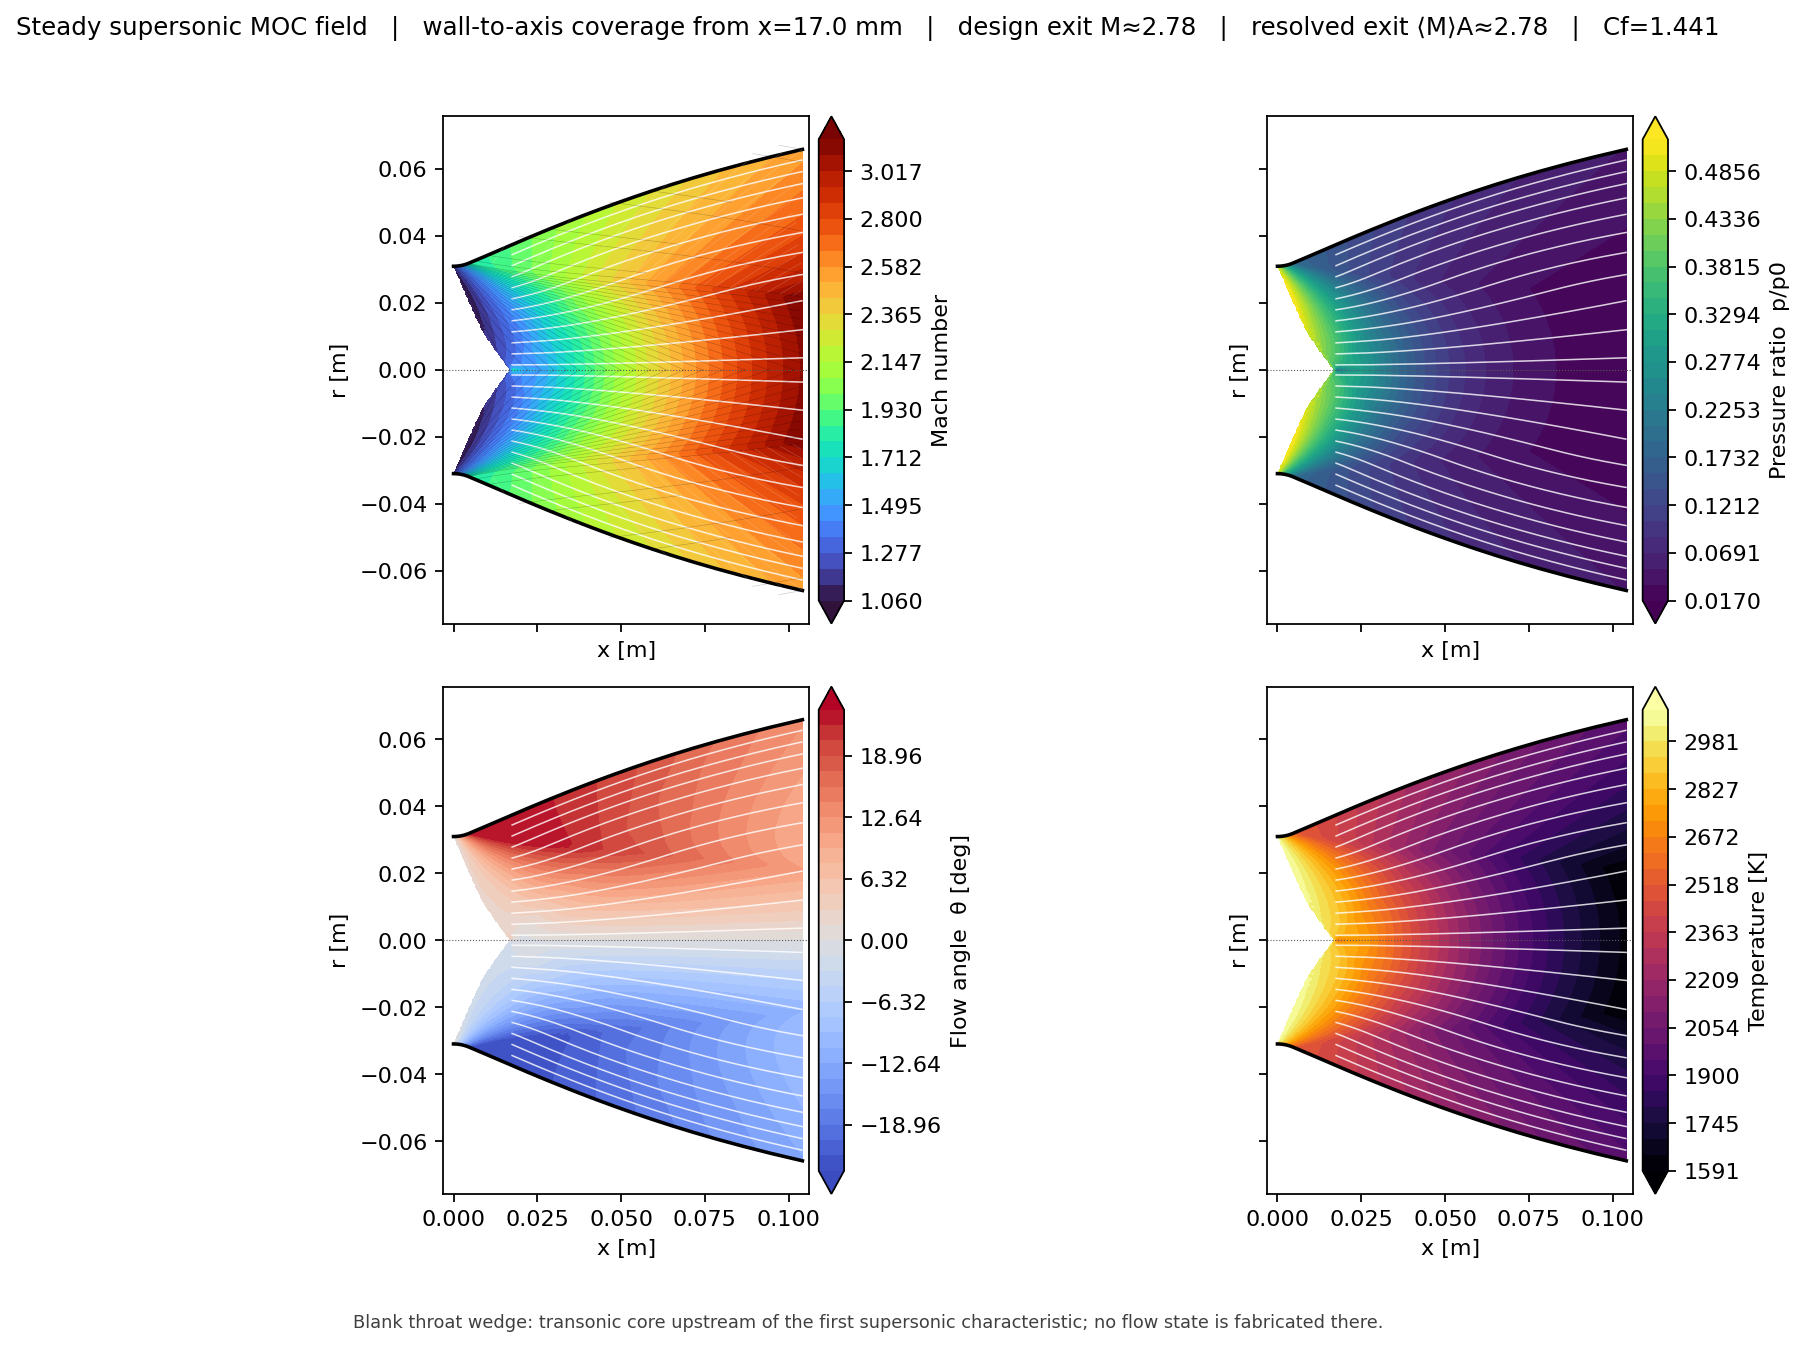
\includegraphics[width=0.58\linewidth,keepaspectratio]{figures/fresh/fresh_13kn_moc_flowfield_mach_p_theta_T.png}\caption{Fresh 2026-11-05 run of examples/cli/test\_13kn\_rao\_bvp\_flowfield.args: the coverage-gated field from flow\_viz.plot\_flowfield. The temperature panel uses -{}-chamber-temp (default 3500 K), not the resolved 3571 K in summary.json.}\label{fig:s12-flowfield}\end{figure}

\subsection{Governing documents}

No triaged document has S12 as its primary stage. \code{docs/subsystems/S06-rao-moc-bvp-contour/REWRITE_PLAN.md} \S12 (Phase 13; plan, no STATUS head) specified the \code{plotting.py} diagnostics; \code{docs/subsystems/S06-rao-moc-bvp-contour/MOC_MARCH_TOPOLOGY_REMEDIATION_2026-09-21.md} (active) has \code{flow_viz} and \code{moc_diagrams} consume the bounded net; \code{injector_pintle_provenance.md} (S08) lists the injector figures and \code{regen_wall_model.md} (S07) the cooling equations.

\subsection{Verification}

\code{tests/test_flow_viz.py} (9 tests): field nodes, rendering, physical ranges, partial-field rejection, BDE coverage, exit mean from the last populated cut, net required, both animations. \code{tests/test_moc_diagrams.py} (7): stashed artifacts, five diagrams with their panels, BDE artifacts required. \code{tests/test_plotting.py} (21): the \S12 diagnostics, bad-link flagging, and the cooling, coolant-march, structural (sourced $N_f$), cross-section and separation figures. \code{tests/test_injector.py:1127} and \code{tests/test_jax_sensitivities.py:127} cover two more figures. None compares images or values with a reference.

\subsection{Maturity, limitations and known defects}

\begin{itemize}
\item \textbf{Chamber temperature.} \code{flowfield.png} and \code{anim_particles.gif} use \code{args.chamber_temp}, never set from thermochemistry (fresh run: \code{performance.Tc_K} = 3571~K against the 3500~K default). The field inherits the constant-$\gamma$ MOC assumption.
\item \textbf{Buckling panel never drawn.} No caller passes \code{buckling_profile} to \code{plot_structural_life_dashboard}, so its second panel always shows the eq.~4-31 margin, never the eq.~4-29 buckling comparison its docstring describes.
\item \textbf{Schematic versus machined STEP.} \code{plot_pintle_schematic} uses the reference layout, so its claim that drawing, tables ``and the solids agree'' does not cover the default machined STEP (\code{resolve_coaxial_layout}).
\end{itemize}

\subsection{Developer notes}

Add a CLI figure as a guarded call beside its stage, with a render test; keep the coverage gate and the no-synthetic-wall rule in \code{flow_viz.py}; change \code{bde_artifacts}, \code{moc_diagrams} and \code{flow_viz} together; never put physics in \code{plotting.py}.
